\section{MLP的训练与应用}

\subsection{反向传播算法}

MLP的训练主要依赖于反向传播算法。该算法包括以下步骤:
\begin{enumerate}
    \item 前向传播
    \item 计算损失
    \item 反向传播误差
    \item 更新权重
\end{enumerate}

对于均方误差损失函数,权重更新的公式可以表示为:

\begin{equation}
    \mathbf{W} = \mathbf{W} - \eta \frac{\partial L}{\partial \mathbf{W}}
\end{equation}

其中,$\eta$是学习率,$L$是损失函数。

\subsection{MLP的应用领域}

MLP在多个领域都有广泛应用,包括但不限于:
\begin{itemize}
    \item 图像识别
    \item 语音识别
    \item 自然语言处理
    \item 金融预测
\end{itemize}

\begin{figure}
    \centering
    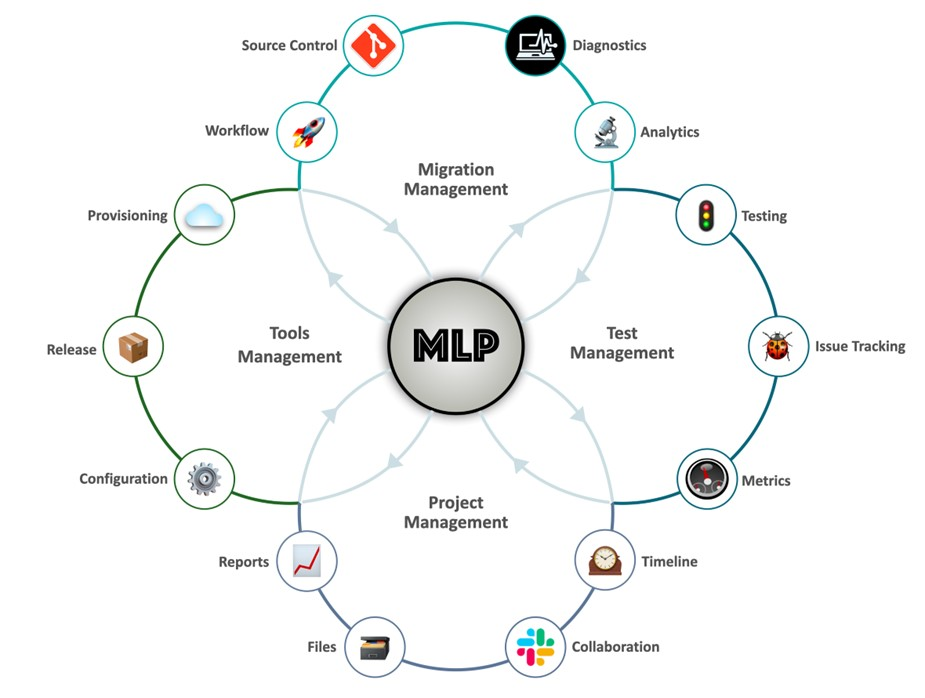
\includegraphics[width=0.8\textwidth]{mlp_application.jpg}
    \caption{MLP在图像识别中的应用示例}
    \label{fig:mlp_application}
\end{figure}

图~\ref{fig:mlp_application}展示了MLP在图像识别任务中的应用示例。

\subsection{MLP的优缺点}

MLP作为一种经典的神经网络模型,有其独特的优势和局限性\cite{LeCun2015}。表~\ref{tab:mlp_pros_cons}总结了MLP的主要优缺点。

\begin{table}
    \centering
    \begin{tabular}{p{0.4\textwidth}p{0.4\textwidth}}
    \toprule
    优点 & 缺点 \\
    \midrule
    能够学习非线性关系 & 可能陷入局部最优 \\
    适用于多种类型的数据 & 对于某些复杂任务,可能需要大量隐藏层和神经元 \\
    结构简单,易于理解和实现 & 容易过拟合,需要careful调参和正则化 \\
    \bottomrule
    \end{tabular}
    \caption{MLP的优缺点}
    \label{tab:mlp_pros_cons}
\end{table}

\subsection{深入学习资源}

要深入学习MLP和其他深度学习模型,可以参考以下资源:

\begin{itemize}
    \item Coursera上的深度学习课程:\url{https://www.coursera.org/specializations/deep-learning}
    \item FastAI的实践课程:\url{https://course.fast.ai/}
    \item TensorFlow官方教程:\url{https://www.tensorflow.org/tutorials}
\end{itemize}

这些资源提供了从理论到实践的全面指导,适合不同层次的学习者。
